\documentclass[12pt,a4paper]{article}
\usepackage[margin=1in]{geometry}
\usepackage{amsmath,amssymb}
\usepackage{booktabs}
\usepackage{caption}
\usepackage{enumitem}
\usepackage{float}
\usepackage{fancyhdr}
\usepackage{graphicx}
\usepackage{hyperref}
\usepackage{longtable}
\usepackage{array}
\usepackage{tabularx}
\usepackage{tikz}
\usepackage{xcolor}
\usepackage{setspace}
\usetikzlibrary{arrows.meta,positioning,shapes.geometric,calc}
\hypersetup{colorlinks=true,linkcolor=blue,urlcolor=blue,citecolor=blue}
\setlength{\parskip}{0.6em}
\setlength{\parindent}{0pt}
\onehalfspacing
\setlength{\headheight}{15pt}
\pagestyle{fancy}
\fancyhf{}
\rhead{GA-Based Delivery Route Optimizer}
\lhead{Project Report}
\cfoot{\thepage}
\begin{document}
\begin{titlepage}
\centering
{\Large Department of Computer Science and Engineering\par}
{\Large Rajshahi University of Engineering \& Technology\par}
\vspace{1.5cm}
{\huge\bfseries GA-Based Delivery Route Optimizer and Shortest Route Finder\par}
\vspace{0.75cm}
{\large A Project Report on Live Route Search, Multi-Stop Optimization, and Map-Based Visualization\par}
\vspace{1.5cm}
\begin{tabular}{rl}
\textbf{Course Code:} & \textnormal{[Course Code]} \\
\textbf{Course Title:} & Machine Learning Sessional \\
\textbf{Submitted by:} & \textnormal{[Your Name]} \\
\textbf{ID:} & \textnormal{[Your Student ID]} \\
\textbf{Submitted to:} & \textnormal{[Teacher Name]} \\
\textbf{Department:} & Department of Computer Science and Engineering \\
\textbf{University:} & Rajshahi University of Engineering \& Technology \\
\textbf{Submission Date:} & 23 April 2026 \\
\end{tabular}
\vfill
{\large \textit{Prepared in the context of a live Streamlit application integrated with OpenStreetMap-based routing services and a Genetic Algorithm optimization engine.}\par}
\end{titlepage}

\newpage
\thispagestyle{empty}
\begin{center}
{\Large Certificate / Approval Page\par}
\vspace{1.25cm}
This is to certify that the project report entitled\par
\vspace{0.5cm}
{\bfseries GA-Based Delivery Route Optimizer and Shortest Route Finder}\par
\vspace{0.5cm}
has been prepared by [Your Name], ID [Your Student ID], under my supervision in partial fulfillment of the requirements for the course Machine Learning Sessional.
\vspace{1.5cm}
\end{center}

\begin{tabular}{p{0.48\textwidth}p{0.48\textwidth}}
\textbf{Signature of Supervisor:} & \textbf{Signature of Student:} \\
\rule{0pt}{1.25cm} & \rule{0pt}{1.25cm} \\
\hrulefill & \hrulefill \\
\textnormal{[Teacher Name]} & \textnormal{[Your Name]} \\
Designation / Department & \textnormal{Student ID} \\
\end{tabular}

\vfill
\begin{center}
Department of Computer Science and Engineering\par
Rajshahi University of Engineering \& Technology\par
Rajshahi, Bangladesh\par
\end{center}

\newpage
\section*{Acknowledgement}
\addcontentsline{toc}{section}{Acknowledgement}
I would like to express my sincere gratitude to my course teacher for guidance, constructive feedback, and evaluation support throughout the development of this project. I am also thankful to the faculty members and classmates who helped me refine the idea into a practical application.

Special appreciation goes to the open-source community and the maintainers of Streamlit, Folium, OpenStreetMap, OSRM, and Nominatim. Their tools made it possible to transform a route optimization concept into a live, interactive system with geolocation, autocomplete search, and map visualization.

Finally, I am grateful to my family and friends for their encouragement and patience during the development and reporting process.

\newpage
\section*{Abstract}
\addcontentsline{toc}{section}{Abstract}
This project addresses the practical problem of finding a good delivery route between a source and a destination, and extending the same system to multi-stop route optimization. In many real-world scenarios such as food delivery, courier dispatch, ambulance movement, and ride sharing, choosing the best route is not only a matter of shortest distance but also of speed, reliability, and ease of use.

The developed application combines a Streamlit front end, browser-based live geolocation, destination autocomplete, and OpenStreetMap-based road routing services. For single source-destination requests, the application finds drivable road routes and displays up to three ranked alternatives on a map. For multi-stop scenarios, a Genetic Algorithm is used to search for a near-optimal visiting order among a fixed set of locations. The algorithm is suitable because the route-ordering problem grows quickly with the number of stops and becomes difficult to solve exactly using brute force.

The project uses tournament selection, ordered crossover, swap mutation, and elitism to evolve better route orders across generations. Fitness is based on inverse route cost, where lower total distance implies higher fitness. The final system presents the selected route visually on an interactive map and also reports road distance and estimated travel time. The outcome is a practical route optimizer that is useful for academic demonstration as well as for small logistics-style decision support.

\newpage
\tableofcontents
\newpage
\listoffigures
\newpage
\listoftables
\newpage
\pagenumbering{arabic}

\section{Introduction}
\subsection{Background}
Route optimization is a core problem in transportation, logistics, and service delivery. A small change in path choice can affect fuel usage, delivery time, customer satisfaction, and operational cost. Modern users also expect route systems to be interactive, location-aware, and easy to understand on a map rather than only as a numerical answer.

\subsection{Problem Statement}
Given a source location, a destination, and optionally several intermediate stops, the system must identify a valid road route or route order that minimizes total travel cost while respecting practical constraints such as road connectivity and fixed start/end points. In the single-source and single-destination case, the application must also show readable route alternatives instead of only one path.

\subsection{Motivation}
The project is motivated by common real-world use cases such as food delivery, logistics dispatch, parcel movement, ride sharing, and emergency response. In these domains, a route should not only exist mathematically; it must be usable on the road network, visible to the user, and fast enough to compute during interaction.

\subsection{Objectives}
The project objectives are:
\begin{itemize}[leftmargin=1.5em]
    \item accept a live source location or a custom searched source,
    \item accept destination and optional stop locations using autocomplete,
    \item generate road-aware routes using map service integration,
    \item optimize stop ordering with a Genetic Algorithm,
    \item show the result on an interactive map,
    \item report route distance, duration, ranking, and diversity.
\end{itemize}

\subsection{Scope of the Project}
This project covers live location detection, road route search, route ranking, multi-stop order optimization, and visualization. It does not include vehicle capacity planning, time-window scheduling, real-time traffic ingestion, or fleet-level dispatch optimization.

\subsection{Report Organization}
Section 2 reviews related work. Section 3 defines the problem. Section 4 describes the complete system architecture. Section 5 explains the methodology and Genetic Algorithm design. Section 6 summarizes implementation details. Section 7 presents the experimental setup. Section 8 discusses results and analysis. Sections 9 to 11 discuss practical value, limitations, future work, and conclusion.

\section{Literature Review / Related Work}
\subsection{Route Optimization Problem}
Route optimization has long been studied in the context of the shortest path problem, the traveling salesman problem, and vehicle routing problems. The difficulty increases significantly when the number of stops rises or when road constraints and real map data must be considered.

\subsection{Traditional Approaches}
\textbf{Dijkstra's algorithm} is a classic shortest path method for non-negative edge weights. It is reliable for one-source and one-destination road search, but it does not directly solve route ordering for many stops.

\textbf{A* search} improves efficiency by using a heuristic estimate to guide exploration. It is especially useful when a reasonable heuristic is available, but it still focuses on graph search rather than combinatorial route ordering.

\textbf{Greedy methods} choose the nearest next point at each step. They are fast and simple, but they can easily get trapped in locally good choices that lead to a worse total route.

\textbf{Brute force search} evaluates all permutations and guarantees the optimum. However, its factorial complexity makes it impractical beyond a small number of stops.

\subsection{Metaheuristic Approaches}
Metaheuristic methods are popular for large combinatorial problems because they provide good approximate solutions in reasonable time. Genetic Algorithm, Simulated Annealing, and Ant Colony Optimization are common examples.

\textbf{Genetic Algorithm} searches by maintaining a population of candidate solutions and applying selection, crossover, and mutation.

\textbf{Simulated Annealing} explores neighboring solutions and accepts occasional worse candidates to escape local minima.

\textbf{Ant Colony Optimization} builds routes using pheromone-inspired probabilistic search and is effective for path problems but often needs careful parameter tuning.

\subsection{Why Genetic Algorithm for This Project}
Genetic Algorithm is suitable for this project because the multi-stop route problem has a large search space and practical constraints. GA can handle permutation-based solutions, produce near-optimal routes, and adapt to future extensions such as time penalties, capacity penalties, or additional business rules. It is also easy to visualize and explain in an academic setting.

\section{Problem Formulation}
\subsection{Input Definition}
The system accepts:
\begin{itemize}[leftmargin=1.5em]
    \item one fixed start location or live current location,
    \item one final destination,
    \item optional intermediate stops for multi-stop optimization,
    \item coordinate data obtained from map-based geocoding services.
\end{itemize}

\subsection{Output Definition}
The expected outputs are:
\begin{itemize}[leftmargin=1.5em]
    \item the best route order or best road path,
    \item total road distance,
    \item estimated travel time,
    \item ranked alternatives when available,
    \item a visual map with route lines and markers.
\end{itemize}

\subsection{Assumptions}
The current system assumes a static or mostly stable road network during route computation. It uses a fixed set of input points and does not deeply model live traffic variation. Road distance and time are derived from external map routing services.

\subsection{Constraints}
The solution must respect:
\begin{itemize}[leftmargin=1.5em]
    \item each location should be visited at most once in a multi-stop route,
    \item the start location is fixed,
    \item the end destination is fixed,
    \item all selected paths must follow valid roads,
    \item route generation should remain fast enough for interactive use.
\end{itemize}

\section{System Overview}
\subsection{Overall System Architecture}
Figure~\ref{fig:architecture} summarizes the complete system.

\begin{figure}[H]
\centering
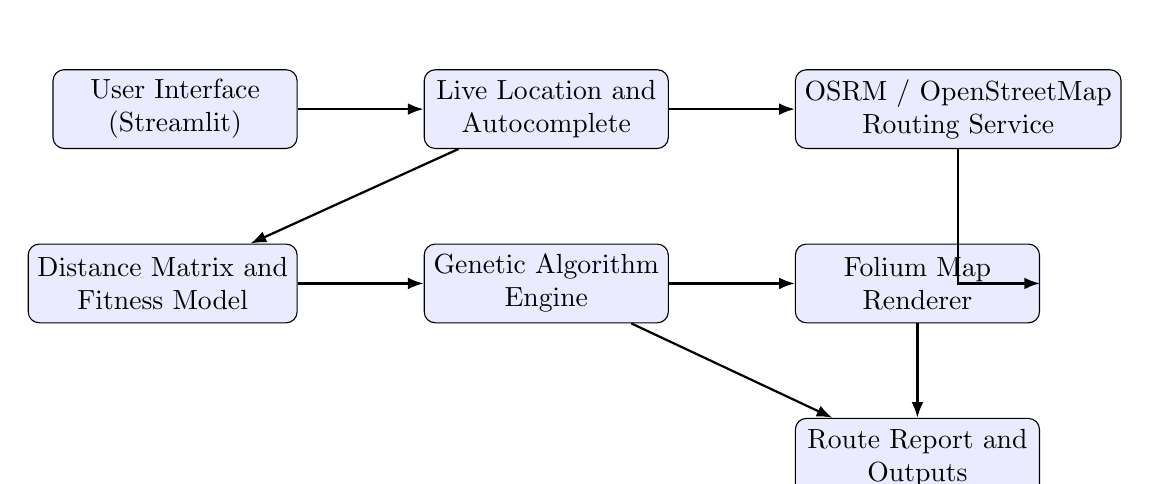
\begin{tikzpicture}[
    node distance=1.2cm and 1.6cm,
    box/.style={draw, rounded corners, align=center, minimum width=3.1cm, minimum height=1cm, fill=blue!8},
    arrow/.style={-{Latex[length=2mm]}, thick}
]
\node[box] (user) {User Interface\\(Streamlit)};
\node[box, right=of user] (geo) {Live Location and\\Autocomplete};
\node[box, right=of geo] (routing) {OSRM / OpenStreetMap\\Routing Service};
\node[box, below=of geo] (ga) {Genetic Algorithm\\Engine};
\node[box, left=of ga] (matrix) {Distance Matrix and\\Fitness Model};
\node[box, right=of ga] (map) {Folium Map\\Renderer};
\node[box, below=of map] (report) {Route Report and\\Outputs};

\draw[arrow] (user) -- (geo);
\draw[arrow] (geo) -- (routing);
\draw[arrow] (geo) -- (matrix);
\draw[arrow] (matrix) -- (ga);
\draw[arrow] (ga) -- (map);
\draw[arrow] (routing) |- (map);
\draw[arrow] (map) -- (report);
\draw[arrow] (ga) -- (report);
\end{tikzpicture}
\caption{Overall architecture of the route optimizer system.}
\label{fig:architecture}
\end{figure}

\subsection{Workflow of the System}
The workflow is straightforward:
\begin{enumerate}[leftmargin=1.5em]
    \item The user selects the source, either as live current location or as a searched place.
    \item The user enters the destination using live autocomplete suggestions.
    \item Coordinates are resolved using the geocoding layer.
    \item Road distance and travel time are fetched from the routing layer.
    \item For multi-stop use cases, a distance matrix is prepared.
    \item The Genetic Algorithm searches for a better stop order.
    \item The final route is rendered on the map with summary metrics.
\end{enumerate}

% \begin{figure}[H]
% \centering
% \begin{tikzpicture}[
%     node distance=1cm and 1.2cm,
%     step/.style={draw, rounded corners, align=center, minimum width=3.4cm, minimum height=0.9cm, fill=green!8},
%     arrow/.style={-{Latex[length=2mm]}, thick}
% ]
% \node[step] (start) {Start};
% \node[step, below=of start] (input) {User selects source / destination};
% \node[step, below=of input] (coords) {Convert places to coordinates};
% \node[step, below=of coords] (matrix2) {Build route cost / distance matrix};
% \node[step, below=of matrix2] (ga2) {Run Genetic Algorithm};
% \node[step, below=of ga2] (best) {Choose best route order};
% \node[step, below=of best] (render) {Render map and metrics};
% \node[step, below=of render] (end) {End};
% \draw[arrow] (start) -- (input);
% \draw[arrow] (input) -- (coords);
% \draw[arrow] (coords) -- (matrix2);
% \draw[arrow] (matrix2) -- (ga2);
% \draw[arrow] (ga2) -- (best);
% \draw[arrow] (best) -- (render);
% \draw[arrow] (render) -- (end);
% \end{tikzpicture}
% \caption{Workflow of the route optimization system.}
% \label{fig:workflow}
% \end{figure}

\subsection{Tools and Technologies Used}
\begin{itemize}[leftmargin=1.5em]
    \item Python for application logic and optimization.
    \item Streamlit for the interactive web front end.
    \item OpenStreetMap ecosystem for map-based location search and road routing.
    \item Folium for interactive map rendering.
    \item Genetic Algorithm modules for stop ordering.
    \item LaTeX for professional report preparation.
\end{itemize}

\section{Methodology}
\subsection{Why Genetic Algorithm Was Chosen}
GA was selected because the route-ordering problem is combinatorial, scalable, and difficult to solve exactly for larger inputs. A direct exhaustive search becomes infeasible very quickly. GA is a practical compromise: it does not guarantee a global optimum, but it can find a strong near-optimal solution in a controlled amount of time.

\subsection{Chromosome Representation}
A chromosome is represented as a permutation of stop indices. For example, if the locations are A, B, C, D, and E, then one chromosome may be \([A, C, B, D, E]\). This sequence defines the visiting order.

\subsection{Population Initialization}
The initial population is created by taking the base ordering and shuffling it randomly multiple times. This produces diverse candidate solutions at the beginning of the search.

\subsection{Fitness Function}
The fitness function is based on route cost. In the current project, lower total distance implies higher fitness. A simple normalized relation is used conceptually:
\[
\text{fitness} = \frac{1}{\text{cost}}
\]
where cost may include distance and optional penalties. This encourages the algorithm to prefer shorter and more efficient routes.

\subsection{Selection Strategy}
The implementation uses tournament selection. A small group of individuals is sampled from the population, and the best among them is selected as a parent. This strategy is simple, robust, and does not require global fitness normalization.

\subsection{Crossover Strategy}
The project uses ordered crossover. This is suitable for route problems because chromosomes are permutations and must not contain repeated stops. Ordered crossover preserves relative order information while still mixing parent solutions.

\subsection{Mutation Strategy}
The mutation operator uses swap mutation. Two positions in the route sequence are exchanged. This helps maintain diversity and allows the population to escape local minima.

\subsection{Elitism}
Elitism is used to retain the best individuals from one generation to the next. This prevents the algorithm from losing high-quality solutions due to random crossover or mutation.

\subsection{Stopping Criteria}
The algorithm stops after a fixed maximum number of generations. In a more advanced version, additional stopping conditions such as no improvement for several generations can also be used.

\subsection{Route Cost Evaluation Logic}
Route cost is evaluated using map-based distance data. For a route order, the system sums the pairwise road costs between consecutive stops. In the live single-destination view, the road service provides distance and estimated duration directly for the selected path.

\subsection{Final Best Route Selection}
The final best route is the chromosome with the highest fitness, which corresponds to the smallest total cost among the evolved candidates. That route is then converted into a map-friendly output and visualized to the user.

\section{Algorithm Design and Logic}
\subsection{Step-by-Step GA Logic}
\begin{enumerate}[leftmargin=1.5em]
    \item Generate an initial population of random stop orders.
    \item Evaluate the cost of each route order.
    \item Convert route cost into fitness.
    \item Select parent routes using tournament selection.
    \item Apply ordered crossover to produce children.
    \item Mutate children with swap mutation.
    \item Keep the best individuals using elitism.
    \item Repeat for the configured number of generations.
    \item Return the best route discovered during the search.
\end{enumerate}

\subsection{Pseudocode of the Algorithm}
\begin{verbatim}
Input: location list L, distance matrix D, GA parameters
Output: best route order R*

1. Initialize population P with random permutations of L
2. Evaluate fitness for every chromosome in P
3. Repeat for each generation:
4.     Preserve elite chromosomes
5.     While new population is not full:
6.         Select parent1 using tournament selection
7.         Select parent2 using tournament selection
8.         Perform ordered crossover to create children
9.         Mutate children using swap mutation
10.        Add children to new population
11.    Replace P with new population
12.    Track best chromosome found so far
13. Return chromosome with highest fitness as R*
\end{verbatim}

\subsection{Flowchart of the GA Process}
The process is already illustrated conceptually in Figure~\ref{fig:workflow}. In practice, the flow is: initialize population, evaluate, select, crossover, mutate, repeat, and finally return the best solution.

\subsection{Time Complexity Discussion}
For a population size $P$, generations $G$, chromosome length $n$, and route-cost evaluation proportional to the number of segments, the total runtime is roughly proportional to $O(G \cdot P \cdot n)$. The exact cost depends on the route evaluation method and whether real map service calls are cached. Compared with brute force, GA is much more practical for moderate and larger problem sizes.

\section{Implementation Details}
\subsection{Folder Structure}
The project is organized into modules for the app, routing, map integration, core optimization, utilities, tests, configuration, and reports. This structure keeps the application maintainable and easier to extend.

\begin{verbatim}
route-optimizer-project/
  app.py
  config/
  data/
  map_integration/
  models/
  outputs/
  report/
  routing_logic/
  src/
  tests/
\end{verbatim}

\subsection{Frontend Design}
The front end is built in Streamlit. The user can detect current location, choose a custom source, search for a destination using live autocomplete, and generate the route in one workflow. The interface is intentionally simple because route tools should minimize friction during user interaction.

\subsection{Map Integration}
The map layer uses Folium and OpenStreetMap tiles. Road routes are rendered as polylines, and source/destination markers are displayed clearly. Multiple alternative routes are assigned different colors so that ranking can be understood visually.

\subsection{Live Location Handling}
Browser permission is used to request current location. If direct geolocation is unavailable, the system can fall back to approximate IP-based location. This ensures the app remains usable even when browser permissions are restricted.

\subsection{Autocomplete and Suggestion Logic}
The source and destination search fields support live suggestions. As the user types, the application queries a geocoding service and presents nearby matching places. This reduces input errors and makes the application feel responsive.

\subsection{Route Generation Logic}
After the source and destination are selected, the routing module queries a road routing service to compute the path. For the live view, up to three ranked route alternatives are returned when possible. The best route is shown first, together with distance and estimated time.

\subsection{Integration of GA with Map Data}
The Genetic Algorithm uses route-cost information derived from the map layer. Once the best ordering is found, the route is passed back to the visualization layer so it can be rendered and reported in a user-friendly way.

\section{Experimental Setup}
\subsection{Test Environment}
The project was developed and tested on a Windows machine using a Python virtual environment and a modern browser for live location permission and map interaction. Streamlit was used as the local web server.

\subsection{Parameter Settings of GA}
Table~\ref{tab:ga-params} lists the GA settings used in the project.

\begin{table}[H]
\centering
\caption{Genetic Algorithm parameter settings used in the project.}
\label{tab:ga-params}
\begin{tabular}{ll}
\toprule
Parameter & Value \\
\midrule
Population size & 80 \\
Number of generations & 150 \\
Mutation rate & 0.12 \\
Crossover rate & 0.90 \\
Elitism count & 4 \\
Tournament size & 4 \\
Random seed & 42 \\
\bottomrule
\end{tabular}
\end{table}

\subsection{Test Cases}
The project can be tested with:
\begin{itemize}[leftmargin=1.5em]
    \item small routes with only a few stops,
    \item medium-size delivery sequences,
    \item larger stop sets to observe GA behavior,
    \item live source-destination searches with map visualization.
\end{itemize}

\subsection{Evaluation Metrics}
The main metrics are total distance, estimated travel time, convergence speed, route diversity, and overall route quality.

\section{Results and Analysis}
\subsection{Output Screenshots}
The application produces interactive map output, route summaries, ranking tables, and live location indicators. Screenshots from the Streamlit app can be inserted into the figures folder later if required for final submission.

\subsection{Sample Route Results}
A typical result includes the best road route, two or more alternatives when available, total distance in kilometers, and estimated travel time in minutes. For multi-stop optimization, the best stop order can also be reported.

\subsection{Convergence Behavior}
In a GA run, the best fitness generally improves across generations and then stabilizes. This indicates that the population is converging toward a strong near-optimal route order.

\subsection{Comparison with Non-Optimized Route}
A non-optimized route often follows arbitrary ordering and can be longer or slower. The GA-based route improves the sequence by searching the permutation space more systematically.

\begin{table}[H]
\centering
\caption{Illustrative comparison between a random route and the GA-based route.}
\label{tab:comparison}
\begin{tabularx}{\textwidth}{lXX}
\toprule
Metric & Random / Unoptimized Route & GA-Based Optimized Route \\
\midrule
Route order & Arbitrary & Evolved by fitness search \\
Total distance & Usually higher & Lower or near-minimal \\
Travel time & Unstable & More efficient \\
Decision quality & Weak & Strong near-optimal \\
Scalability & Poor for many stops & Better for moderate stop counts \\
\bottomrule
\end{tabularx}
\end{table}

\subsection{Discussion of Results}
The system is practically useful because it combines optimization, live routing, and visualization in one interactive workflow. The route ranking and diversity panels improve interpretability by showing why one route is preferred over another. The approach is stable for small and medium-sized route sets and is appropriate for academic demonstration.

\section{Practical Value and Present Perspective}
\subsection{Real-World Applications}
The project is relevant to food delivery, logistics, courier services, ambulance routing, and ride sharing.

\subsection{Present-Day Value Addition}
It can reduce fuel usage, lower delivery time, improve customer satisfaction, and increase operational efficiency.

\subsection{Business Perspective}
Companies can use similar routing tools to reduce operating cost and improve service quality. Even a small percentage of route improvement can matter when many deliveries are processed every day.

\subsection{User Perspective}
Users get a faster and smarter route recommendation experience, along with a map-based explanation of the selected path.

\subsection{Academic Perspective}
The project demonstrates a full combination of metaheuristic optimization, live web application design, and geospatial routing. That makes it a strong academic example of applied machine learning-style optimization.

\section{Limitations of the Current System}
\begin{enumerate}[leftmargin=1.5em]
    \item No real-time traffic awareness is integrated.
    \item The system depends on external routing and geocoding services.
    \item GA provides near-optimal, not guaranteed globally optimal, solutions.
    \item Some practical constraints such as vehicle capacity or time windows are not yet modeled.
    \item Performance can drop if the number of stops becomes very large.
\end{enumerate}

\section{Future Improvements}
\begin{enumerate}[leftmargin=1.5em]
    \item Integrate real-time traffic and congestion data.
    \item Add time-window constraints for delivery scheduling.
    \item Support vehicle capacity constraints and multi-vehicle routing.
    \item Combine GA with local search or other hybrid optimization methods.
    \item Improve the UI/UX for stronger production readiness.
    \item Add a mobile application version.
    \item Learn from historical routes using machine learning.
\end{enumerate}

\section{Conclusion}
This project solved the route optimization problem by combining live road routing with Genetic Algorithm-based search for route ordering. The live Streamlit application can detect source location, accept searched destinations, compute road routes, rank alternatives, and display them on a map with distance and estimated time. For multi-stop scenarios, the GA engine provides a scalable and flexible near-optimal solution.

The main contribution of the project is not only the algorithm itself but also its integration into a usable interactive system. This makes the work practical, demonstrable, and extensible for future logistics and transportation applications.

\begin{thebibliography}{99}
\bibitem{goldberg}
D. E. Goldberg, \textit{Genetic Algorithms in Search, Optimization, and Machine Learning}. Addison-Wesley, 1989.

\bibitem{cormen}
T. H. Cormen, C. E. Leiserson, R. L. Rivest, and C. Stein, \textit{Introduction to Algorithms}. MIT Press, 2009.

\bibitem{dorigo}
M. Dorigo and L. M. Gambardella, ``Ant Colony System: A Cooperative Learning Approach to the Traveling Salesman Problem,'' \textit{IEEE Transactions on Evolutionary Computation}, vol. 1, no. 1, pp. 53--66, 1997.

\bibitem{streamlitdoc}
Streamlit Documentation. Available: \url{https://docs.streamlit.io/}

\bibitem{osrmdoc}
Open Source Routing Machine Documentation. Available: \url{https://project-osrm.org/}

\bibitem{nominatimdoc}
Nominatim Documentation. Available: \url{https://nominatim.org/}
\end{thebibliography}

\appendix
\section{Appendix A: Full Pseudocode}
\begin{verbatim}
Procedure GA_Route_Optimization
Input: list of stops S, distance matrix D, GA parameters
Output: best visiting order R*

Create initial population P
Evaluate each chromosome using total route cost
For generation = 1 to max_generation do
    Keep elite chromosomes
    While population is incomplete do
        Select parents using tournament selection
        Apply ordered crossover
        Apply swap mutation
        Add children to next population
    End While
    Replace old population with new population
    Update the best chromosome found so far
End For
Return the chromosome with best fitness
\end{verbatim}

\section{Appendix B: Important Code Snippets}
The project uses a permutation-based GA with ordered crossover and swap mutation. The core idea is to keep valid stop orders and improve them over generations.

\begin{verbatim}
fitness = 1 / route_cost
parents = tournament_selection(population)
child = ordered_crossover(parent1, parent2)
child = swap_mutation(child)
\end{verbatim}

\section{Appendix C: Additional Screenshots}
You may place final app screenshots, route maps, and convergence plots in the report figures folder and include them here if your teacher requests visual evidence.

\section{Appendix D: Parameter Tables}
The main GA parameter table is already included in Section 7.2. Additional experiment-specific parameter tables can be inserted here if needed.

\end{document}
